\documentclass[11pt,a4paper]{article}
\usepackage[T1]{fontenc}
\usepackage[margin=2.3cm]{geometry}
\usepackage{amsmath,amssymb}
\usepackage{graphicx}
\usepackage[dvipsnames]{xcolor}
\usepackage{enumitem}
\usepackage[colorlinks=true,linkcolor=blue,urlcolor=blue]{hyperref}
\setlength{\parskip}{0.6em}
\setlength{\parindent}{0pt}
\begin{document}

\begin{center}{\LARGE\bfseries openclassifier}\\[0.4em]{\large Draw decision boundaries and read a confusion matrix, in three sessions.}\\[0.2em]\small PAN IIT OSS explainer \textbullet{} higher secondary to advanced undergraduate (levels 4-6)\end{center}

\section*{Why this exists}
Every automatic decision, from a spam filter to a screening test, is a classifier: a rule that splits cases into groups. This explainer shows how such rules are drawn and, more importantly, how to judge them honestly, using only counting, a few formulas and Python.

\section*{The end goal}
Draw decision boundaries and read a confusion matrix. The end goal is to draw decision boundaries and read a confusion matrix: to see what a classifier decides, to count how it fails, and to ask the right questions (what is the base rate, what do the mistakes cost, was this tested on new data) before trusting a number. All examples use synthetic data and are for education only.

\section*{How the three sessions build up}
\begin{enumerate}[nosep]
\item \textbf{Session 1: A rule that splits two groups} (Level 1, conceptual interactive model, 60 min).
\item \textbf{Session 2: Trees, neighbours and the confusion matrix} (Level 2, mathematical engineering model, 90 min).
\item \textbf{Session 3: Judging a classifier honestly} (Level 3, simulation and validation, 90 min).
\end{enumerate}

\section{Session 1: A rule that splits two groups}

\subsection*{A. Real-world problem}
A packing line must send ripe fruit to the shop and keep unripe fruit back. A camera measures two numbers for each fruit: its size in centimetres and a colour score from 0 (green) to 10 (deep red). Nobody tells the machine what ripe means; we give it a rule. How should the rule look, how do we draw it, and how do we count the ways it goes wrong? (General education with made-up data.)

\subsection*{B. Concept and theory}
A classifier is a rule that maps measurements to a class. Each fruit is a point (x, y) = (size, colour). The simplest rule asks one question about one number: is the size above t? A better rule mixes both numbers: it calls a fruit ripe when x cos(a) + y sin(a) is greater than c. The set of points where the answer flips is the decision boundary, here a straight line; the angle a says which way the line faces and c says how far it sits from the origin. Call 'ripe' the positive class. A rule can go wrong in two different ways: a false alarm (false positive) calls an unripe fruit ripe, and a miss (false negative) calls a ripe fruit unripe. They are counted separately because they usually cost different amounts. Sliding the boundary towards the ripe cluster removes false alarms but creates misses, and the other way round.

\begin{itemize}[nosep]
\item x: fruit size (cm)
\item y: colour score (0 green to 10 red) (score units)
\item a: angle of the boundary's normal direction (degrees)
\item c: offset of the boundary from the origin (score units)
\item FA: false alarms: unripe fruit called ripe (count)
\item miss: ripe fruit called unripe (count)
\end{itemize}

\begin{equation*}
\text{called ripe}\iff x\cos a+y\sin a>c
\end{equation*}

\begin{equation*}
\text{size-only rule}:\ \text{called ripe}\iff x>t
\end{equation*}

\begin{equation*}
\text{accuracy}=\frac{\text{number correct}}{\text{number of fruit}}
\end{equation*}

\begin{center}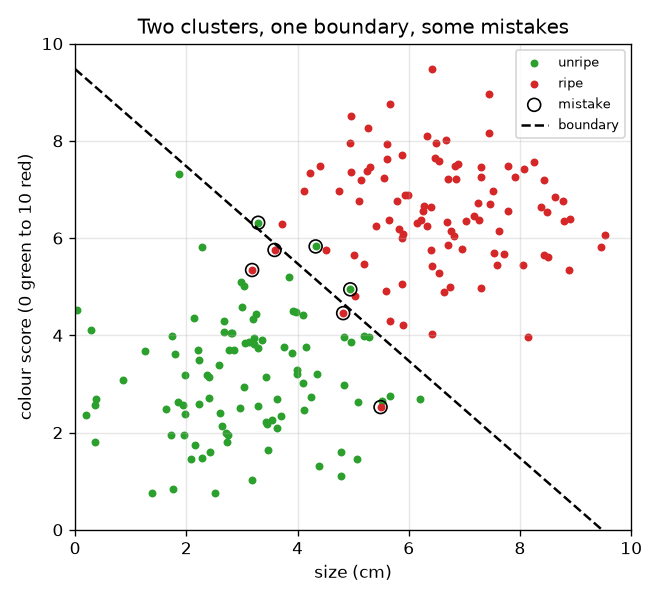
\includegraphics[width=0.85\linewidth]{figures/s01_clusters_boundary.png}\\\small Two overlapping clusters, a dashed boundary, and rings around the fruit the rule gets wrong.\end{center}

\subsection*{E. Worked example}
Twelve fruit: unripe (2, 2), (3, 4), (4, 2), (3.5, 6), (5, 3), (6, 4.5) and ripe (4.5, 7), (6, 8), (7, 6), (8, 9), (7.5, 4), (5.5, 5.5). Use the line with a = 45 degrees and c = 7. Which fruit are misclassified, and what is the accuracy?
\begin{enumerate}[nosep]
\item At 45 degrees cos = sin = 0.7071, so the rule is 0.7071 (x + y) \textgreater{} 7, that is x + y \textgreater{} 9.899.
\item Sums x + y for the unripe fruit: 4, 7, 6, 9.5, 8, 10.5. Only 10.5 (the fruit at (6, 4.5)) is above 9.899, so it is a false alarm.
\item Sums for the ripe fruit: 11.5, 14, 13, 17, 11.5, 11. All are above 9.899, so there are no misses.
\item Correct = 12 - 1 - 0 = 11, so accuracy = 11 / 12 = 0.917.
\end{enumerate}
\textbf{Answer.} One false alarm (the fruit at (6, 4.5)), no misses, accuracy 0.917.

\subsection*{F. Questions}
\begin{enumerate}[nosep]
\item \textbf{Conceptual.} Why do we count false alarms and misses separately instead of just counting 'mistakes'? Give an example where one is worse than the other.
\item \textbf{Numerical.} For the twelve fruit of the worked example, use the size-only rule 'ripe if size \textgreater{} 5' (that is a = 0 degrees, c = 5). Count the false alarms, the misses and the accuracy.
\item \textbf{Graph and simulation interpretation.} In the trade-off graph for 200 random fruit with the 45 degree boundary, what happens to the two counts as the offset c increases from 2 to 11? Where do they cross?
\item \textbf{Design and optimisation challenge.} Design: the shop says a false alarm (unripe fruit on the shelf) is worse than a miss. Should you move the boundary left or right of c = 6.7? What do you give up? How would you decide how far?
\end{enumerate}

\section{Session 2: Trees, neighbours and the confusion matrix}

\subsection*{A. Real-world problem}
A screening test for a rare condition is described as 'more than 99 percent reliable'. You test positive. How worried should you be? Surprisingly, the honest answer can be 'about one chance in six', and the reason is not the test but how rare the condition is. To see why, we need a classifier that outputs a decision, a table that counts its four outcomes, and Bayes' rule. (General education only, with made-up numbers: never personal medical advice.)

\subsection*{B. Concept and theory}
A decision tree classifies by asking a chain of yes/no questions of the form 'is feature j at most t?'. Which question? The one that makes the two resulting groups as pure as possible. For a group with a fraction p1 of class 1 and p0 = 1 - p1 of class 0, the Gini impurity is 1 - p0\textasciicircum{}2 - p1\textasciicircum{}2: 0 for a pure group and 0.5 for a 50/50 group. A split is scored by the weighted Gini of the two halves, and the best split is found by trying every feature and every midpoint between sorted values. Repeat inside each half down to a maximum depth; a depth-1 tree is a stump. k nearest neighbours keeps all the training points and votes among the k closest ones to a new point: small k gives a ragged boundary, large k a smooth one. The confusion matrix counts true positives (TP), false positives (FP), false negatives (FN) and true negatives (TN). Accuracy = (TP + TN) / total, precision = TP / (TP + FP) (of those flagged, how many were right), recall = TP / (TP + FN) (of the real positives, how many were found), and F1 = 2 TP / (2 TP + FP + FN), the harmonic mean of precision and recall. For a test with sensitivity (recall on positives) and specificity (rate of correct negatives) applied to a population with prevalence q, Bayes' rule gives the positive predictive value PPV = q sens / (q sens + (1 - q)(1 - spec)). When mistakes cost different amounts, give a score and call a case positive at or above a threshold; if the score were the true probability p, calling positive is cheaper when p is above c\_fp / (c\_fp + c\_fn).

\begin{itemize}[nosep]
\item p1: fraction of class 1 in a group (no unit)
\item G: Gini impurity of a group (no unit)
\item k: number of neighbours in the vote (count)
\item TP, FP, FN, TN: confusion matrix counts (count)
\item q: prevalence: fraction of the population that has the condition (no unit)
\item sens, spec: sensitivity and specificity of the test (no unit)
\item c\_fn, c\_fp: cost of a miss and of a false alarm (cost units)
\end{itemize}

\begin{equation*}
G = 1 - p_0^2 - p_1^2
\end{equation*}

\begin{equation*}
G_{\text{split}} = \frac{n_L\,G_L + n_R\,G_R}{n_L+n_R}
\end{equation*}

\begin{equation*}
\text{precision}=\frac{TP}{TP+FP},\quad \text{recall}=\frac{TP}{TP+FN},\quad F_1=\frac{2TP}{2TP+FP+FN}
\end{equation*}

\begin{equation*}
\text{PPV}=\frac{q\cdot\text{sens}}{q\cdot\text{sens}+(1-q)(1-\text{spec})}
\end{equation*}

\begin{equation*}
\text{call positive when } p>\frac{c_{fp}}{c_{fp}+c_{fn}}
\end{equation*}

\begin{center}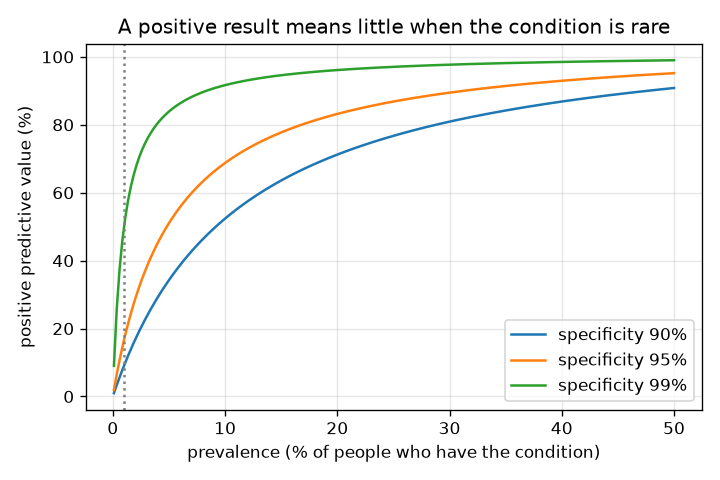
\includegraphics[width=0.85\linewidth]{figures/s02_base_rate.png}\\\small Positive predictive value against prevalence for three specificities: rare conditions give low PPV.\end{center}

\subsection*{E. Worked example}
A condition has prevalence 1 percent. The test has sensitivity 99 percent and specificity 95 percent. Of 10000 people tested, how many test positive, and what fraction of those truly have the condition?
\begin{enumerate}[nosep]
\item Have the condition: 1 percent of 10000 = 100 people. The test finds 99 percent of them: TP = 99, FN = 1.
\item Do not have it: 9900 people. The test wrongly flags 5 percent of them: FP = 0.05 x 9900 = 495, and TN = 9900 - 495 = 9405.
\item Everyone who tests positive: 99 + 495 = 594 people.
\item PPV = 99 / 594 = 0.1667, about 16.7 percent. By Bayes: 0.01 x 0.99 / (0.01 x 0.99 + 0.99 x 0.05) = 0.0099 / 0.0594 = 0.1667. The two methods agree.
\item The overall accuracy is (99 + 9405) / 10000 = 95.04 percent, yet five of every six positives are false alarms.
\end{enumerate}
\textbf{Answer.} 594 people test positive, only 99 of them truly have the condition: PPV = 16.7 percent.

\subsection*{F. Questions}
\begin{enumerate}[nosep]
\item \textbf{Conceptual.} A friend says: 'The test is 95 percent accurate, so a positive result means a 95 percent chance of having the condition.' What is wrong with this?
\item \textbf{Numerical.} A classifier produces TP = 40, FP = 10, FN = 20 and TN = 130 on 200 cases. Compute accuracy, precision, recall and F1.
\item \textbf{Graph and simulation interpretation.} On the PPV graph at prevalence 1 percent, what PPV do specificities of 90, 95 and 99 percent give (sensitivity 99 percent)? At what prevalence does a 95 percent specificity reach a PPV above 80 percent?
\item \textbf{Design and optimisation challenge.} Design: a miss costs 10 units and a false alarm costs 1 unit. You have a classifier that gives scores between 0 and 1. Why should the threshold be below 0.5, how low would the theory put it if the scores were true probabilities, and how should you choose it in practice?
\end{enumerate}

\section{Session 3: Judging a classifier honestly}

\subsection*{A. Real-world problem}
A model that scores 100 percent on its own training data can fail on new cases; a model can be accurate overall while flagging one group of people far more often than another; and a model can look brilliant only because of a bookkeeping slip. How do we judge a classifier honestly? The tools are held-out data, the ROC curve, cross-validation, group-wise error rates, and a habit of asking how a number could be fooling us. (All data are synthetic; nothing here says anything about real people.)

\subsection*{B. Concept and theory}
Most classifiers output a score and call a case positive at or above a threshold. Lower the threshold and the true-positive rate TPR = TP / (TP + FN) rises, but so does the false-positive rate FPR = FP / (FP + TN). The ROC curve plots TPR against FPR for every threshold; the area under it (AUC) equals the probability that a randomly chosen positive case scores higher than a randomly chosen negative case (ties count one half). A random forest averages many trees, each grown on a bootstrap sample (n cases drawn with replacement) and combined by majority vote; individual trees are unstable but their vote is steadier. A deeper tree can memorise noise: its training accuracy rises to 100 percent while accuracy on new data falls. K-fold cross-validation shuffles the cases into k folds and, for each fold, trains on the rest and tests on that fold, so every case is tested once. A score is calibrated if, among cases scored near 0.7, about 70 percent are positive. For fairness, compare error rates by group: if group B's scores are all shifted up by s but the ranking inside each group is the same, then with one threshold t the false-positive rates are 1 - Phi(t) and 1 - Phi(t - s), different even though AUC is equal. Two failure cases: leakage (using test data when scaling or choosing features inflates accuracy) and class imbalance (accuracy hides a useless classifier when positives are rare).

\begin{itemize}[nosep]
\item TPR: true-positive rate (recall) (no unit)
\item FPR: false-positive rate (no unit)
\item AUC: area under the ROC curve (no unit)
\item t: decision threshold on the score (score units)
\item d: separation between class centres, in score spreads (no unit)
\item s: upward shift of group B's scores (score units)
\item Phi: the standard normal cumulative distribution function (no unit)
\item k: number of cross-validation folds (count)
\end{itemize}

\begin{equation*}
\text{TPR}=\frac{TP}{TP+FN},\qquad \text{FPR}=\frac{FP}{FP+TN}
\end{equation*}

\begin{equation*}
\text{AUC}=\int_0^1 \text{TPR}\,d(\text{FPR})=P\big(\text{score}_{+}>\text{score}_{-}\big)
\end{equation*}

\begin{equation*}
\text{FPR}_A=1-\Phi(t),\qquad \text{FPR}_B=1-\Phi(t-s),\qquad \text{TPR}_g=1-\Phi(t-s_g-d)
\end{equation*}

\begin{equation*}
\text{AUC}=\Phi\!\left(\frac{d}{\sqrt{2}}\right)
\end{equation*}

\begin{center}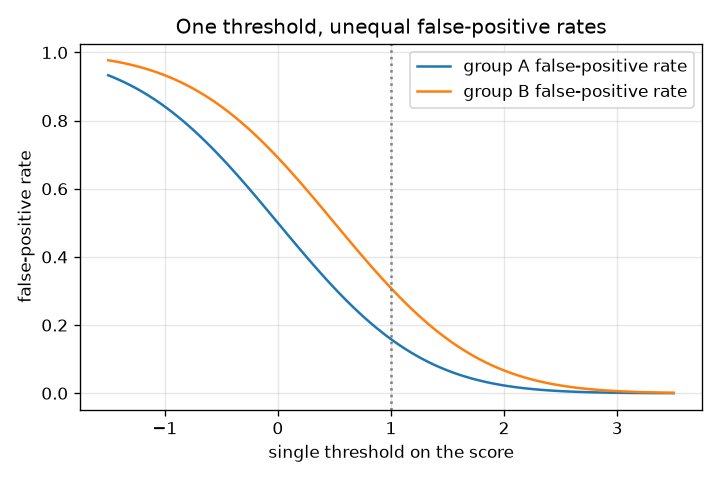
\includegraphics[width=0.85\linewidth]{figures/s03_fairness.png}\\\small One threshold, two groups: the false-positive rate curves are parallel but apart.\end{center}

\subsection*{E. Worked example}
Four cases have scores 0.1, 0.4, 0.35, 0.8 and true labels 0, 0, 1, 1. Build the ROC curve and compute the AUC by area and as a probability.
\begin{enumerate}[nosep]
\item Sort by score, highest first: 0.8 (positive), 0.4 (negative), 0.35 (positive), 0.1 (negative). There are 2 positives and 2 negatives.
\item Lower the threshold past each score and update (FPR, TPR): start (0, 0); after 0.8 -\textgreater{} (0, 0.5); after 0.4 -\textgreater{} (0.5, 0.5); after 0.35 -\textgreater{} (0.5, 1); after 0.1 -\textgreater{} (1, 1).
\item Area under the curve by trapezoids: 0 + 0.5 x 0.5 + 0 + 0.5 x 1 = 0.25 + 0.5 = 0.75.
\item Pairs (positive, negative): 0.35 \textgreater{} 0.1 yes, 0.35 \textgreater{} 0.4 no, 0.8 \textgreater{} 0.1 yes, 0.8 \textgreater{} 0.4 yes: 3 of 4 pairs, probability 0.75. The two methods agree.
\end{enumerate}
\textbf{Answer.} AUC = 0.75, both from the area under the ROC curve and as the probability that a random positive outranks a random negative.

\subsection*{F. Questions}
\begin{enumerate}[nosep]
\item \textbf{Conceptual.} Why can training accuracy reach 100 percent while test accuracy falls as a tree gets deeper? Why does a forest of trees help?
\item \textbf{Numerical.} Group B's scores are shifted up by 0.5 relative to group A, negatives are centred at 0 and the threshold is 1.0. Compute each group's false-positive rate with Phi(1) = 0.8413 and Phi(0.5) = 0.6915.
\item \textbf{Graph and simulation interpretation.} In the overfitting figure, which depth would you choose and why? What does the gap between the two curves tell you?
\item \textbf{Design and optimisation challenge.} Design: a screening problem has 5 percent positives; a miss costs 20 and a false alarm costs 1. You may choose a depth-3 tree, a depth-8 tree or a 25-tree forest and a threshold. Which would you pick and how do you justify it?
\end{enumerate}

\section{Real-world mini-project}
\textbf{Choose a model and a threshold for a synthetic screening problem.} A clinic-style screening problem, entirely synthetic: 5 percent of cases are positive, a miss costs 20 units and a false alarm costs 1 unit. Use \texttt{make\_screening}, \texttt{grow\_tree}, \texttt{fit\_forest}, \texttt{pick\_threshold} and \texttt{cost\_and\_confusion} from Session 3. For each of three models (a depth-3 tree, a depth-8 tree and a 25-tree forest of depth 6), choose the threshold that minimises the cost on a validation set, then report the confusion matrix and the cost on a separate test set. General education only: this is not a medical tool.

\section{The path ahead}
\begin{enumerate}[nosep]
\item \textbf{Session 4: Tune the forest by cross-validation.} A forest whose depth is chosen by your own cross-validation loop.
\item \textbf{Session 5: A threshold for each group.} A tool that picks one threshold per group and reports both groups' error rates.
\item \textbf{Session 6: Beat the screening cost.} A screening classifier chosen and tuned only with validation data.
\item \textbf{Session 7: How sure is the AUC?.} A 95 percent bootstrap interval for the AUC and a coverage experiment.
\item \textbf{Session 8: Three classes and a 3 by 3 confusion matrix.} A classifier for three fruit types with a 3 by 3 matrix and macro-F1.
\end{enumerate}

\section{Answers and hints}

\subsection*{Session 1}
\begin{enumerate}[nosep]
\item \textbf{Conceptual.} Hint: Think about what each mistake costs the packing line. Solution: Both are wrong decisions, but they cost different things. Sending an unripe fruit to the shop (false alarm) loses a customer's trust; keeping a ripe fruit back (miss) wastes a good fruit. For a smoke alarm a miss (fire, no alarm) is far worse than a false alarm. The total number of mistakes hides this, so we report both.
\item \textbf{Numerical.} Hint: List the sizes of the unripe fruit and the ripe fruit and mark which are above 5. Solution: Unripe sizes: 2, 3, 4, 3.5, 5, 6; only 6 is above 5, so 1 false alarm (size exactly 5 is not above 5). Ripe sizes: 4.5, 6, 7, 8, 7.5, 5.5; only 4.5 is not above 5, so 1 miss. Correct = 12 - 2 = 10, accuracy = 10 / 12 = 0.833. Sanity check: using colour as well (the 45 degree line) did better, with only 1 mistake.
\item \textbf{Graph and simulation interpretation.} Hint: A larger c moves the line towards the ripe cluster. Solution: False alarms fall steadily (96 at c = 2, with 0 misses) because fewer fruit are called ripe, and misses rise from 0. The curves cross near c = 6.6, where the two counts are about equal. At c = 6.7 the rule makes 3 false alarms and 4 misses out of 200.
\item \textbf{Design and optimisation challenge.} Hint: Use the trade-off curves: which way does each count move? Solution: Move it right (larger c): fewer false alarms, at the price of more misses, which here means more ripe fruit kept back. To decide how far, give each mistake a cost (for example a false alarm costs 3 and a miss costs 1), compute 3 x FA + 1 x miss along the c axis and take the lowest point. Assumption: the sample is typical of the real line; with only 200 fruit the exact best c is uncertain.
\end{enumerate}

\subsection*{Session 2}
\begin{enumerate}[nosep]
\item \textbf{Conceptual.} Hint: Compare accuracy, specificity and positive predictive value. Solution: Accuracy, sensitivity and specificity describe how the test behaves on people whose true state is known. A positive result asks the reverse question: given the test result, what is the true state? That is the PPV, and it depends on prevalence as well. With 1 percent prevalence the PPV is 16.7 percent even though the overall accuracy is 95.04 percent.
\item \textbf{Numerical.} Hint: Total = 200. Use the four formulas in Section B. Solution: Accuracy = (40 + 130) / 200 = 0.85. Precision = 40 / 50 = 0.8. Recall = 40 / 60 = 0.667. F1 = 2 x 40 / (2 x 40 + 10 + 20) = 80 / 110 = 0.727. Sanity check: F1 lies between precision and recall.
\item \textbf{Graph and simulation interpretation.} Hint: Read the three curves at the x value 1; use the PPV formula to check. Solution: At 1 percent prevalence the PPV is 9.1 percent for specificity 90 percent, 16.7 percent for 95 percent and 50 percent for 99 percent. At 20 percent prevalence a specificity of 95 percent gives a PPV of 83 percent, so the curve passes 80 percent a little below a prevalence of 20 percent. The lesson: improving specificity helps most when the condition is rare.
\item \textbf{Design and optimisation challenge.} Hint: Compare the expected cost of saying positive with that of saying negative; then think about which data you may use to choose. Solution: For a case with true probability p, saying positive costs (1 - p) x 1 and saying negative costs p x 10; positive is cheaper when p \textgreater{} 1 / 11 = 0.0909. Real scores are not perfect probabilities, so search the thresholds on a separate validation set. In the code, a threshold of 4/15 = 0.267 for a k = 15 neighbour classifier gave a test cost of 55, against 90 at the default 0.5. Trade-off: a low threshold buys fewer misses with more false alarms. Assumption: the costs are right and the validation set resembles future cases.
\end{enumerate}

\subsection*{Session 3}
\begin{enumerate}[nosep]
\item \textbf{Conceptual.} Hint: Think about what a leaf holding a single noisy case has learned. Solution: A deep tree keeps splitting until every leaf is pure, so it memorises the training labels, including the noise from flipped labels; that memorised noise does not repeat in new data. A single tree is also unstable: a different training set gives a very different tree. A forest averages many trees grown on bootstrap samples, so the wobble of individual trees partly cancels, and predictions change less from one training set to the next.
\item \textbf{Numerical.} Hint: FPR\_A = 1 - Phi(t) and FPR\_B = 1 - Phi(t - s). Solution: FPR\_A = 1 - Phi(1.0) = 1 - 0.8413 = 0.1587. FPR\_B = 1 - Phi(1.0 - 0.5) = 1 - Phi(0.5) = 1 - 0.6915 = 0.3085. Group B's false-positive rate is about twice group A's. Sanity check: shifting B's scores up pushes more of its negatives over the threshold.
\item \textbf{Graph and simulation interpretation.} Hint: Never choose by training accuracy; read the test curve. Solution: Choose depth 2, where test accuracy peaks (0.7385). Beyond it the training accuracy keeps rising (100 percent by depth 15) while test accuracy falls to 0.6065 at depth 20. The widening gap between the curves is the overfitting. In practice you would pick the depth by cross-validation on the training data, not by looking at the test set.
\item \textbf{Design and optimisation challenge.} Hint: Choose the threshold on a validation set for each model, then compare the models on a separate test set. Solution: For each model pick the cheapest threshold on the validation set, then measure the cost on the test set. On the shipped data the test costs are 1360 (depth 3), 1685 (depth 8) and 1230 (forest), against 2300 for flagging nobody. Pick the forest: the deeper single tree overfits and costs more. Its confusion matrix (TP, FP, FN, TN) is (76, 450, 39, 2435): it accepts many false alarms because they are 20 times cheaper than misses. Assumptions: the costs are right and future data look like the test set.
\end{enumerate}

\section{How to join}
Read \texttt{CONTRIBUTING.md} in the repository, then pick an issue labelled \texttt{good first issue}. Repository: \url{https://github.com/KrunalPanchal1995/openclassifier}

\end{document}
